%=======================================================================================%
\chapter{Review of the Molecular Cause of Cystic Fibrosis and Its Treatment}
\label{chap:cftr_review}
\chapquote{Because of what's inside me; Because of my genes;-Bob Flanagan, "Why."}{}
\newpage
%Authors note:
% We begin with a breif overview of the disease Cystic Fibrosis as it is the main motiation for this project. A horrendous disease for which we will soon find a cure.
% The purpose of this chapter is to present an overview of CFTR's structure and mechanism of action as discovered by a combination of structural and physiological studies. In addition to the actions of CFTR modulators.
\section{Clinical outcomes of Cystic Fibrosis}
Cystic Fibrosis (CF) is the most common fatal genetic condition in Caucasian populations. 165 000 people are afflicted globally. Even with decades of research there is no known cure for CF. With the average life expectancy of patients falling below 50 even in countries with developed health care systems such as the USA and Australia\cite{}\cite{}. The cause is from a build up of salts inside epithelial cells. This causes the surface of the epithelium to dehydrate. When dehydrated the cilia on the epithelium collapse leaving them unable to clear the mucus that naturally lines the airway\cite{boucher2007}. The dehydration mentioned earlier causes the mucus to thicken. This buildup has two pathogenic functions. Firstly it inhibits the normal function of the organ, as mucus fills ducts that would normally pass nutrients in the pancreas or absorb gasses in the lungs. Secondly, the stationary mucus allows bacterial infection, this can further degrade lung function and remains one of the most troublesome chronic complications in CF patients. 

Much of the clinical research into CF has been managing the movement of this mucus and the populations of bacterium in it. Patients often require to hours of physical therapy to help clear this mucus since their lungs are unable to. They must also inhale saline solutions in order to counteract the osmotic pressure in their epithelium. This helps draw more moisture out of the epithelial cells to allow the cilia to move. 

CF patients struggle to intake nutrients due to the build up of mucus in their pancreas and large intestines. This leads to CF related diabetes which afflicts roughly half of adults with CF \cite{Kayani2018}. Patients with CF related diabetes are often administered enzymes and must adhere to a specific diet. A strict diet is particularly important when a patient is taking CFTR modulators because many compounds found in food have interactions with these drugs \cite{}.

\begin{figure}
	\label{CF_life_expectancy}
	\begin{center}
	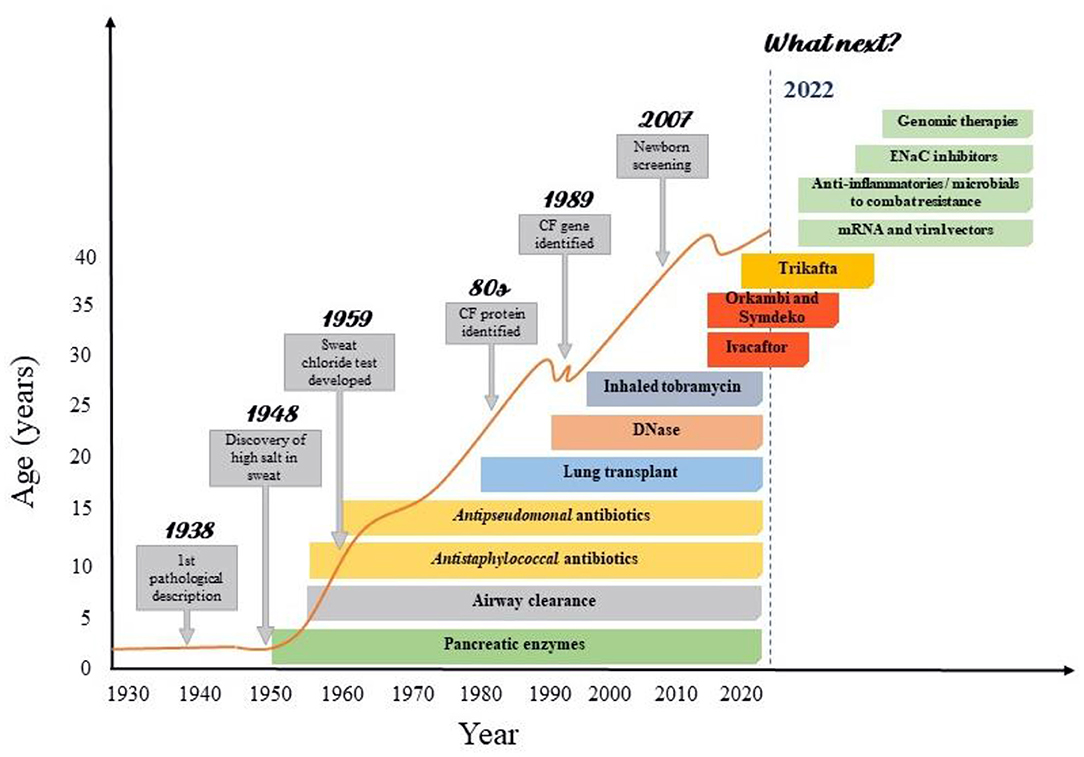
\includegraphics[width=\textwidth]{figures/CF_life_expectancy.png}
	\end{center}
	\captionsetup{singlelinecheck = false, justification=raggedright}
	\caption[CF Clinical Progress] {\textbf{CF Clinical Progress}}{Life expectancy of CF patients correlates highly with translational research. Source \cite{garcia2022}} 
\end{figure}

\section{CFTR Structure}

\begin{figure}
	\label{CFTR_structure_domains}
	\begin{center}
	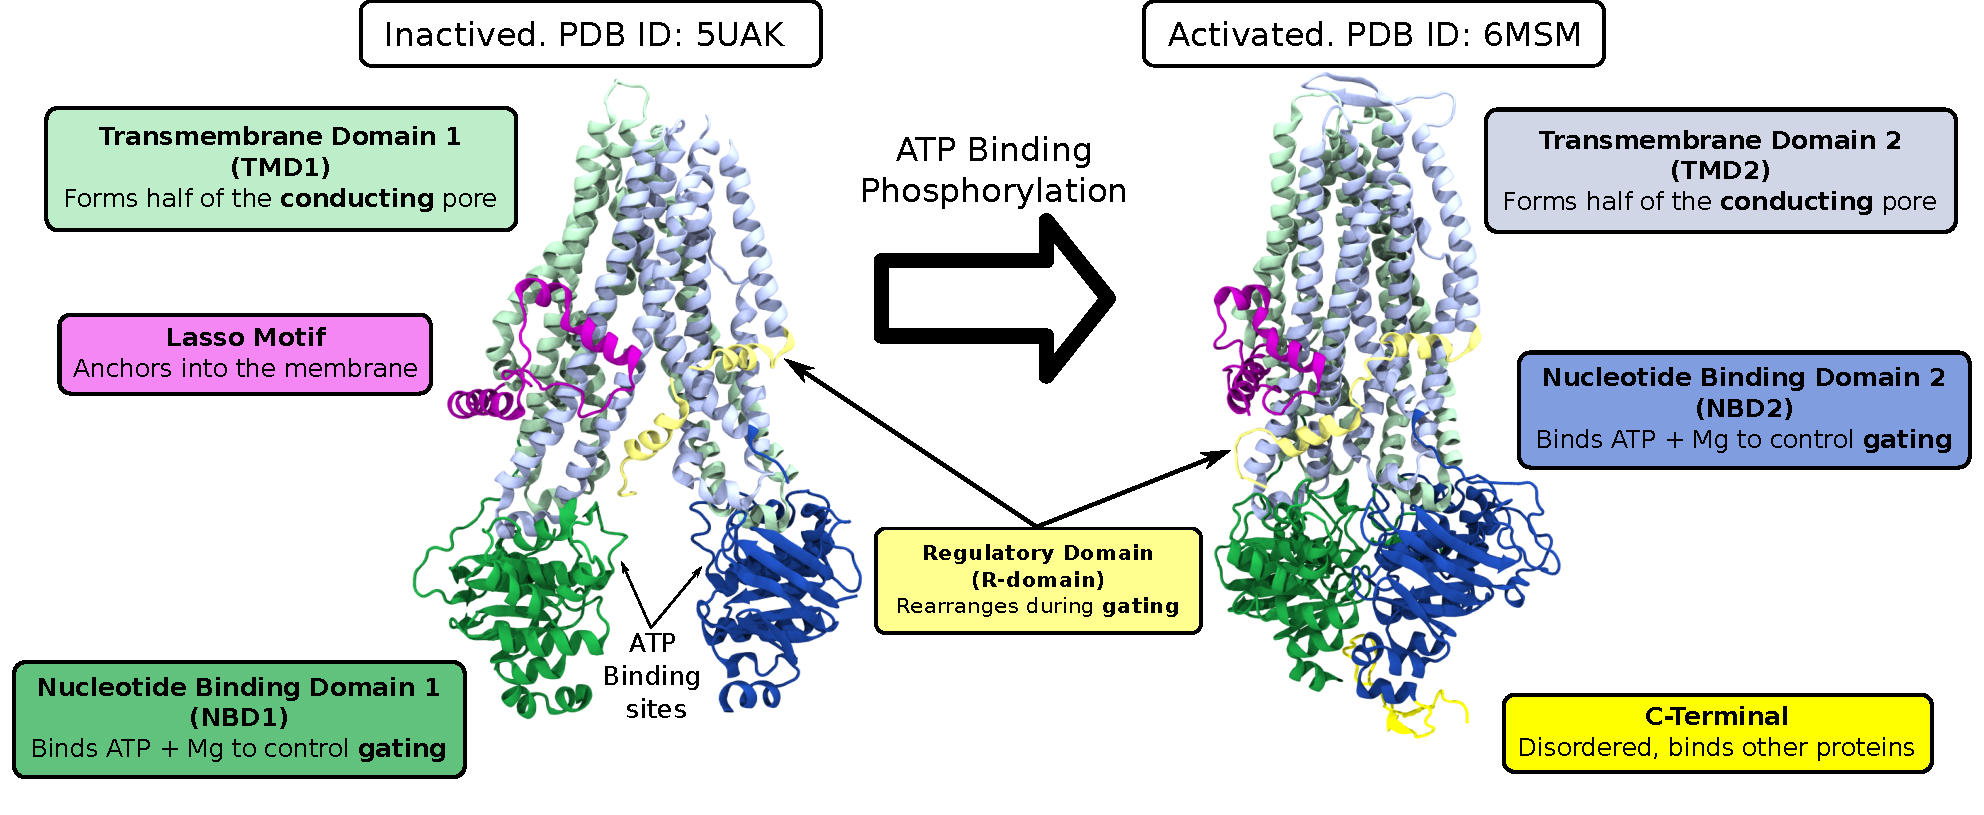
\includegraphics[width=\textwidth]{figures/CFTR_structure.pdf}
	\end{center}
	\captionsetup{singlelinecheck = false, justification=raggedright}
	\caption[CFTR Structure] {\textbf{CFTR Structure}}{CFTR's structure and domains } 
\end{figure}
CFTR is organised into 7 domains (FIGURE). In the order of their primary sequence they are; The Lasso motif, which anchors into the membrane and serves as an interaction hub with other protein partners such as syntaxin and filamin \cite{}. Transmembrane Domain 1 (TMD1) which forms half of the pore. Nucleotide Binding Domain 1 (NBD1) which binds ATP when the channel is in the open state. The Regulatory domain (R-domain) which, when phosphorylated allows the channel to open. Transmembrane domain 2 (TMD2) which forms the other half of the ion conducting pore. Nucleotide Binding Domain 2 

CFTR belongs to a super family of proteins known as ATP Binding Cassette Transporters,  many of these proteins perform active transport across cell membranes. The substrates they transport can vary, including lipids and drug molecules. Proteins in this family share a common motif known as Nucleotide Binding Domains (NBDs). These domains act as ATPases, accelerating the hydrolysis of ATP. The energy from hydrolysis is then transferred into the protein in order for it to pump its substrate against a concentration gradient. 

\section{CFTR is a Unique ABC Transporter}

\begin{figure}
	\label{ABC_diversity}
	\begin{center}
	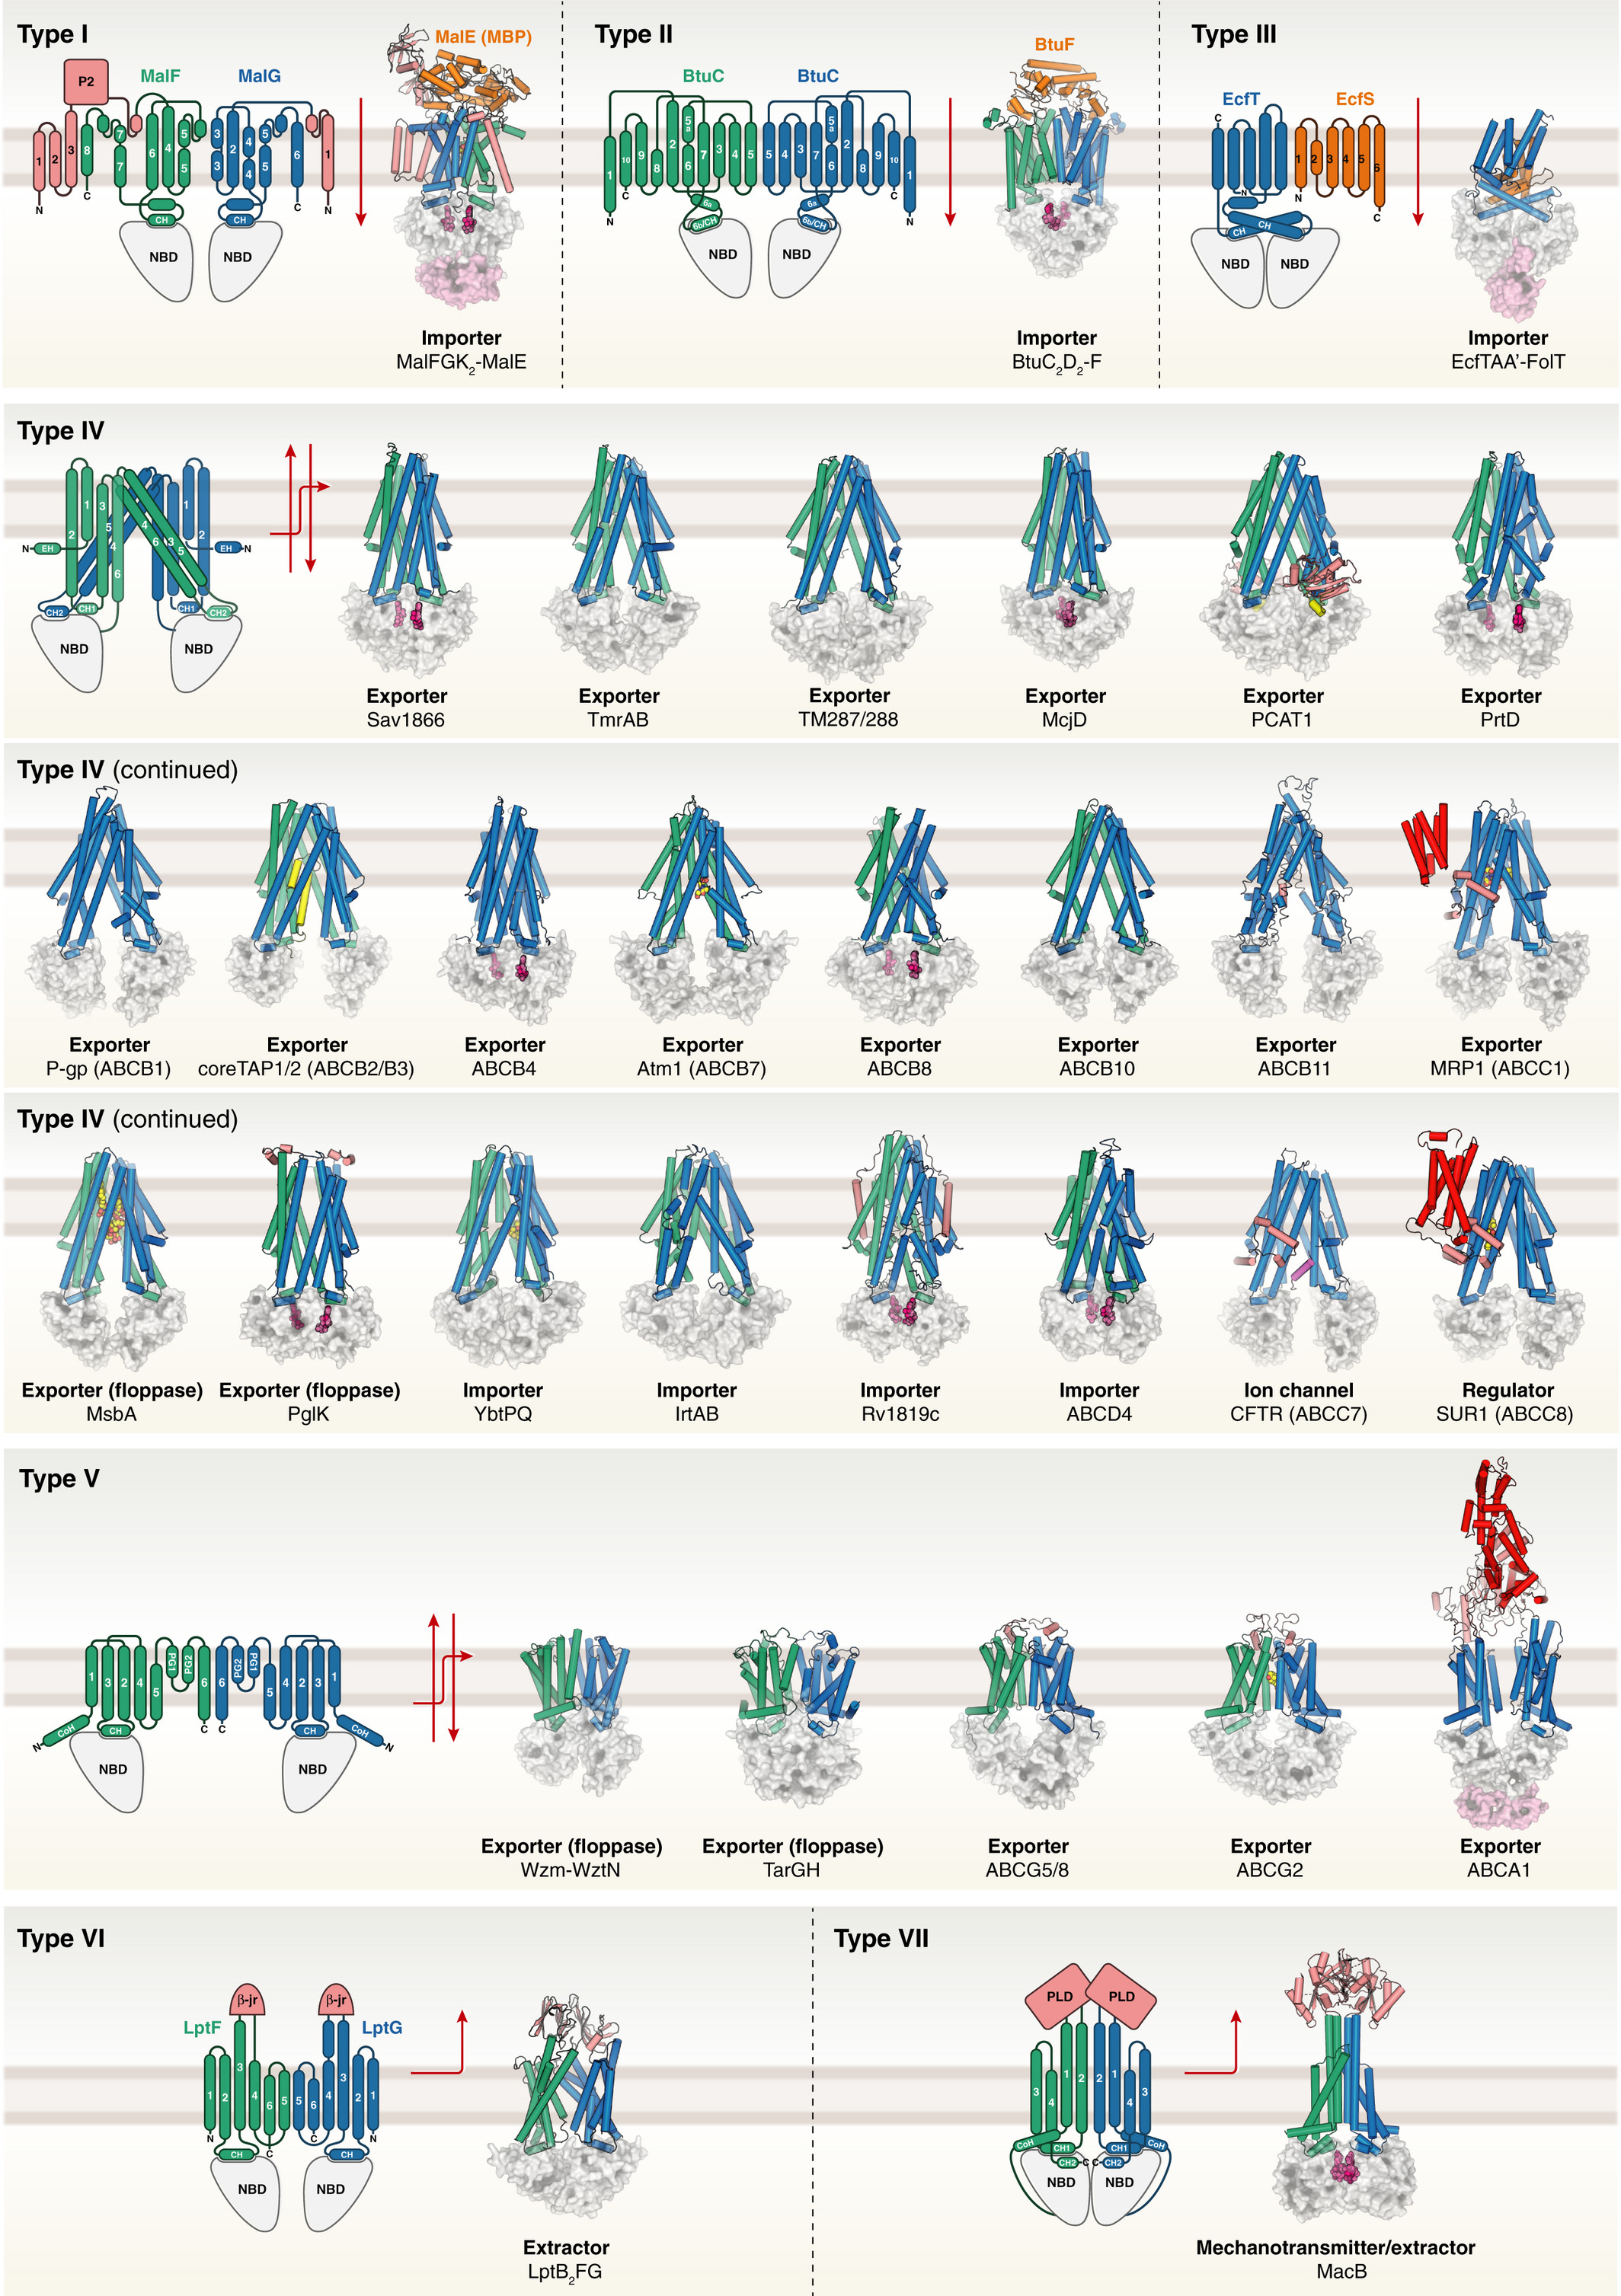
\includegraphics[width=\textwidth]{figures/ABC_classification.png}
	\end{center}
	\captionsetup{singlelinecheck = false, justification=raggedright}
	\caption[CFTR Structure] {\textbf{CFTR Structure}}{The structural diversity of ABC transporters. Structures are classified based on the organisation of their TMDs.\cite{thomas2020}} 
\end{figure}
ATP-Binding Cassette (ABC) transporters are an intriguing super family of proteins. On the whole, they transport substrates by using a combination of phosphorylation energy from ATP hydrolysis. These can be diverse substrates such as lipids or small molecules. Their structural diversity can be seen in figure \ref{ABC_diversity} reflecting their array of functions. 

CFTR is unique, as it is not a transporter, but rather an anion \textit{channel}. The kinetic energy of the ATP is not used to translocate substrate across the membrane but rather simply used in the regulation of the gating cycle. Chloride, bicarbonate and other anions are able to \textit{passively} diffuse through the channel. This evolutionary misappropriation of a transporter to a "leaky channel" is perhaps the reason so many mutations can create a non-functional protein \cite{linsdell2018}.

\section{CFTR classification and structure}

The primary cause of the disease Cystic Fibrosis (CF) is the misfunction of a chloride channel, the Cystic Fibrosis Transmembrane Conductance Regulator (CFTR). This ion channel is a member of the ABCC subfamily of ABC transporters, designated ABCC7. This channel is unique amongst this family because it is not generally considered an active transporter but something of a low conductivity channel or a "weak pump"\cite{linsdell2018}.

CFTR is distinguished by a regulatory region known as the R-domain (residues 645-845) which links NBD1 to TMD2. This region acts to lock the channel in the closed state by wedging itself between the TMDs and dislodging when any one of 3 sites are phosphorylated \cite{mihalyi2020}. In experimentally determined structures of human CFTR the secondary structure of a section of the R-domain but not at high enough resolution to determine the identity of individual side chains \cite{zhang2018}\cite{zhang2016}. Further secondary structure information can be found through experiments with NMR \cite{Baker2007}.

Previous computational studies of CFTR have been used homology models based on the phosphorylated zebra fish protein PDBID:5W81 \cite{zhang2017a}. These have yielded interesting results but the sequence similarity between human and zebrafish CFTR is only 55\% \cite{}. For a protein structure where a single amino acid mutation leads to misfunction, more precision can only help. Additionally, the activity of CFTR modulators is not conserved in mutant zCFTR possibly because it has different kinetics to the human channel \cite{}. In order to do precision medicine we need precision structures. 

An open state of the channel has been proposed by combining both the zebra fish homology model and the fully outward facing conformer of a bacterial ABC transporter Sav1866 \cite{Hoffmann2018}. Although this model has several characteristics expected of the open channel, such as the critical R352-D993 salt bridge, it lacks a salt bridge between R104-E116. In experiments, these residues could be replaced by cysteines and the channel would still function. However, when reducing agents were added to the system the channel lost its ability to open fully. This indicates that in the oxidised environment the C104-C116 cysteines formed a disulfide bridge but its breaking upon exposure to reducing agents caused a loss of function in the channel. This indicates that in the WT channel R104-E116 form a stable salt bridge. 

This salt bridge is clearly visible in the recent cryo-EM structure of ATP-bound human CFTR \cite{zhang2018}.

\section{The Gating Cycle}
The conformational transition from inactive to active differs significantly in CFTR compared to other ABC transporters. The NBDs are largely similar to other to those found in other ABC transporters, they dimerise in what is termed a head to tail configuration so both subunits contact both bound ATP molecules \cite{} See FIGURE. Residue E1371 allows nucleophilic attack on the $\gamma$ phosphate of the ATP bound to Walker B \cite{Stratford2007}. This provides a "kick" to provide the kinetic energy for the opening of the channel CITATION NEEDED. 

\section{Classes of Misfunction to CFTR}
The 360 disease causing mutations to CFTR have been classified into 6 common classes based on the nature of the CF they cause, their reaction to CFTR modulators, and results \textit{in vitro} assays. Ultimately I aim to show that at the atomic level these classes of mutations are less meaningful and as patient specific theratyping evolves these classes will become less relevant, serving as illustrative tools only to communicate at a higher level what is going wrong with the CFTR protein. The canonical classification is as follows:
\begin{itemize}
	\item \textbf{Class I} No functional protein. Under these mutations no protein is transcribed due to either problems with the transcription of mRNA or a premature stop codon truncating protein synthesis early, meaning the resulting peptide is missing key domains. 
	\item \textbf{Class II} Folding defect. These mutations cause the translated peptide to misfold into the incorrect tertiary structure. This can inhibit the protein's journey as it is trafficked to the cell membrane, its function while once it is there or its functional life time at the surface. 
	\item \textbf{Class III} Impaired Gating. Here the mutation inhibits the ability of the protein to transition from the closed to the open state. 
	\item \textbf{Class IV} Decreased Conductance. These mutations cause a barrier in the energy landscape of the CFTR chloride conductance pathway.
	\item \textbf{Class V} Less Protein Expressed.  
	\item \textbf{Class VI} Decreased Lifetime

\end{itemize}

Although useful, in reality this paradigm struggles to reflect the fact that a mutation can belong to multiple categories to different levels due to different modes of pathogenesis. Through our molecular simulations we can see that in reality CFTR modulators are capable of treating several different mutations with very different molecular fingerprints. We will break down this paradigm into more molecular detail in chapter \ref{chap:outlook_review}

FIGURE demonstrates how each of the canonical classes at the molecular level is broken down into many sub classes and a mutation might belong to one of many of these subclasses. Structural biology paradigms and \textit{in silico} modelling can help classify mutations into these different classes. In combination with wet lab assays we can understand which classes of these molecular defects are most effectively treated with specific drug regimens. Our computational microscope is helping choose treatments for patients at the atomic level. 

\section{CFTR Modulators}
Since CF is caused by malfunctions of the channel it makes sense to pursue CFTR as a drug target. Through high throughput \textit{in vitro} screening several (GET NUMBER) compounds have been developed that aim to rescue the function of CFTR. These fall into two classes. Correctors, which aid CFTR to fold into the correct state and potentiators which help the channel reach the fully open state once it has already folded correctly. Emerging evidence suggests that specific genetic defects may be optimally rescued by specific combinations and doses of both correctors and potentiator compounds. Recently, cryo-EM structures of these compounds in their bound state have been released. In addition to several \textit {in vitro} biophysical experiments to determine the precise mechanism of action and binding site of these compounds.

\subsection{Correctors}
The mechanism of action for corrector compounds appears to be to bind to to a pocket between TMH1 and TMH3. Circular dichromism and fluorescence experiments found that an isolated construct of TMH3 and TMH4 were more likely to fold correctly in the presence of corrector compounds. Later cryo-EM structures discovered high resolution electron density in the pocket in the shape of the drug compounds \cite{fiedorczuk2022}. 

In combination this is strong evidence for the precise mechanism of action for corrector compounds. Further work will aid in the creation of new compounds to refine our exploitation of this mechanism.

Mention that there are some interactions between correctors and NBD1.

\subsection{Potentiators}
There is more uncertainty surrounding the mechanism of potentiator drugs. Experiments clearly demonstrate that they act directly on CFTR in order to increase the likelihood that it occupies the open state. They bind to the protein with picomolar affinity. There are are cryo-EM structures which show the drugs bound to the TM8 hinge region \cite{}. \textit {In vitro} experiments suggest at least two membrane facing binding pockets due to the drugs extreme hydrophobicity\cite{}. The location of this second binding site is unknown. The difficulties arise with mutagenesis experiments. The dose-response curves in several studies show that when various sites are mutated the activity of the drug is lowered. This indicates additional binding sites not yet well defined. 

GLPG1837 has not been approved in a clinical setting. \textit {in vitro} experiments suggest that it is more efficacious even though it has lower affinity for CFTR binding (CITATION NEEDED). This would indicate that the highest affinity binding pocket does not produce the greatest modulation. More work is needed to resolve the mechanism which results in the clinical effectiveness of these drugs.  

These drugs are clinically efficacious \cite{VanGoor2014} on several mutants with some curious exceptions like N1303K. I suggest the following mechanism for their action. I suspect a similar analogy exists for the action of the correctors. WT-CFTR exhibits a natural landscape with kinetic barriers in the transition between the closed and open states. A gating class mutation to CFTR will introduce a kinetic barrier in the pathway of this conformational transition. What these drugs do is reduce a barrier in the existing conformational landscape of CFTR. This compensates for the barriers introduced by the mutation. 

This provides a rationale for why it appears possible for diverse range of molecular defects to be treatable by these small molecules. In our work we've found that the atomic nature of the defects introduced by each mutation varies widely, what is interesting is that experiments in \textit{ex vivo} models have shown that these drugs treat a variety of different defects. The classification of classes of defect is outdated, really there are as many classes as there are mutations.


\subsection {Anion Selectivity}
CFTR is weakly selective for specific anions. F337 is the most important amino acid for selectivity. Bicarbonate (HCO$_3^-$ is known to have roughly 26\% the permeability of chloride through the channel. Note that Fluoride has even higher conductance through CFTR, likely due to its small size and high solvation energy (does this indicate hydrated conductance?). WNK1 is known to influence the selectivity of the channel https://www.ncbi.nlm.nih.gov/pmc/articles/PMC6889609/. The permeation of bicarbonate is very important physiologically because if a mutation permeates bicarbonate it means there is a high likelihood the patient will be pancreatic sufficient. 

Compared to cation channels like Gramicidin and KcsA, CFTR is only weakly selective, permeating a large set of annions with varying radii and geometries. Supposedly it is more permeant to lyotropic (low solvation energy annions) rather than cosmotropic anions (high solvation energy annions) indicating that dehydration of the anion is likely during conductance (CITATION NEEDED). The radius of hydrated chloride ions is 3.2A\cite{yang2002} so even with this larger pore partial dehydration must take place. 

\section{Addressing Controversies Surrounding the Structure of CFTR}
The most recent structure of human CFTR in a phosphorylated environment has some interesting features which have lead to some controversies in the literature. After spending significant time researching them I have conducted an extensive literature review in order to learn more about of these concerns. The released structure of activated, human CFTR has two features that have caused some in the CF field to suggest issues with this structure. Firstly, this structure is not sufficiently open to conduct chloride ions. Chloride ions have a diameter of 1.7$\AA$ while the structure has a constriction of 1.1$\AA$\cite{Zhang2018}. So, there must be some level of conformational changes, even if chloride were to move through the channel completely dehydrated. This becomes even more of an issue when considers the experimental evidence where much larger anionic species such as bicarbonate and glutathione were shown to permeate through the channel\cite{kogan2003}. This suggests that there is a much larger conformation which has not been observed experimentally or in simulations. This was the motivation for chapter \ref{chap:opening} of this thesis. Some studies have been performed in order to study the possible permeation paths of chloride but they have not addressed the pressing question of how larger ions might permeate the channel. Bicarbonate in particular is of great physiological importance as there is a high correlation between the channel's ability to permeate bicarbonate and the pancreatic sufficiency of a patient carrying the mutation. In light of this, structural knowledge of a fully open conformation of CFTR is critical to a personalised approach to the treatment of CFTR.

The second and harder to resolve controversy concern the role of TM8. This transmembrane helix has an unusual bend in the middle of the plasma membrane. This is not something seen before in ABC transporters of this type. So it has led to some open questions as to how this bend might contribute to the function of the channel \textit{or} how it might be an artifact of the imaging process. For the former case, the structural biologists in the Chen lab proposed a mechanism whereby the upper hinge of TM8 swings 55$^o$ during the transition to the open state. This mechanism would give justification of the pathogenesis of certain mutaions such as L927P. 

The arguments for the bend in the helix appear to be unphysical. In cryoEM structures, we can observe that the bent conformation is stabilised by salt bridges R347-D924 and E873-R933. The former bond has been well studied experimentally and was expected in the 3d structure. Additionally, all hydrogen bonds along the in the bent helix are . Been observed to be stable in MD \cite{corradi2018} .  is energetically stable.

However, there are still some unanswered questions for the discrepancy between the solved human and solved chicken structures. Certain salt bridges are not present in the latter structure and so single channel electrophysiology experiments may be able to resolve these issues. For example, in 6MSM, the human structure of CFTR there is a salt bridge between amino acids 933 and D873 which is not present in the chCFTR structures. This bond is also present in the zCFTR structure 5W81. If a charge swapped mutant such as R933E/E873R restores WT-like gating behaviour to the channel it would be  strong evidence for the unwound conformation of TM8. 

The two proposed conformations also have vastly different ion permeation pathways, and so blockers engineered to target one conformatoin over the other would also go a long way to answering these questions. The available evidence strongly favors the R334 pathway between TM1 and TM6. Such as experiments to  demonstrate the blockage of current with zinc have shown that mutations to R334 strongly suggest that chloride permeates along this route. Additionally, trhere are several disease causing mutations in the region surrounding R334, such as R334W, R117H, E116K, D110H, I336K\cite{cftr2}. This permeation route also explains the rationale behind the gain of function mutation F337A \cite{}. Determining which model is correct has wide implications for creating the next generation of mutation targeted potentiator class drugs.

A study assessing the accuracy of Alphafold's predictions of transmembrane protein structures found an intersting result. When alphafold made predictions that involved the use of templates it predicts the unwound conformation of TM8. On the other hand, when templates are removed from alphafolds predictions it predicts a straight TM8 conformation, very similar to that found in chCFTR. The authors of this study suggested the reason for the discrepancy was due to the use of detergents in the deteremination of the structure of hCFTR. However, careful reading of cryo-EM literature reveals no examples where the use of detergents has resulted in such drastic conformational changes. One of the few examples where both detergents and native-like nanodisks were used to determine the structure of a protein are the determinations of the structure of TRPV1. These studies revealed no difference to the backbone helices but did suggest important information about the the importrance of different interactions with lipids. A lot of work has been performed in order to create detergents which reflect a native lipid environment and these are the species that were used in . 

The authors of the chCFTR paper suggested that the different expression systems used in the two studies could be the reason for the discrepancy between the two systems, due it their different post translational processing apparatus. Although both groups used mammalian cell lines the chCFTR paper used hamster? cells \cite{aleksandrov2015} and the Chen lab used HEK293S cells. The chicken structure underwent significant mutations in order to be locked open and crystallised. The regulatory insertion was deleted, Many hydrophobic amino acids were introduced into NBD1 in order to aid in the purification of the protein. 

Figure \ref{} shows the large diversity of structures in type IV ABC transporters, many of which also exhibit bends within transmembrane helices. 

\section{Patient Derived Organoids}
The basic unit of living things are cells. In the medical field there is growing capability to discern the functioning of an individual patient's cells. In the field of Cystic Fibrosis Medical Research a recent breakthrough has been to take samples from the epithelium of patients with the disease and grow those samples into tissues which mimic the function of the entire organ\cite{depoel2020}. This is possible in the epithelium due to a population of adult stem cells which maintain the ability to differentiate into a variety of cell types (a property known as pluripotency). 

Adult stem cells in the epithelium are preferable because other sources of stem cells such as induced pluripotent stem cells (iPSCs) require complex, time consuming protocols to grow into fully developed organoids. 

In the case of CF this technology allows the construction of a scalable, patient specific platform where a patient's own tissues can be tested to determine the best treatment for them. These pre-clinical models will allow more patients in the heterogeneous set of disease causing mutations to access modulators. 

Forskolin Induced Swelling (FIS) assays have been used to characterise the patient specific response of a patient's organoids to a drug regimen \cite{dekkers2013}. 


One limitation of these organoid platforms is the lack of an inflammatory response since no immune cells are present in the tissue culture. 


%
